\documentclass{beamer}
\usetheme[sectionpage=none, progressbar=frametitle, numbering=none]{metropolis}        % Use metropolis theme
\usepackage{tikz}
\usetikzlibrary{tikzmark,decorations.pathreplacing,calc}

\title{An Architecture for Task and Traffic Offloading in Edge Computing via Deep Learning}
\date{\today}
\author{Alessandro Gaballo}
\institute{Supervisor: Flavio Esposito - Saint Louis University}


% logo of my university
\titlegraphic{%
  \begin{picture}(0,0)
    \put(290,-135){\makebox(0,0)[rt]{
\includegraphics[width=2.5cm]{img/eurecom_logo}}}
  \end{picture}} 
 
\AtBeginSection[]{
%\frame{\sectionpage}
}

\newcommand{\mytoc}{\frame{\frametitle{Talk overview}\tableofcontents[currentsection,currentsubsection,subsectionstyle=show/shaded/hide, subsubsectionstyle=show/shaded/hide]}}

%subsubsection page
\newcommand{\subsubsectionpage}{
\begin{frame}
  \centering
  \begin{minipage}{22em}
    \raggedright
    \usebeamercolor[fg]{section title}
    \usebeamerfont{section title}
    \insertsectionhead\\[-1ex]
    \usebeamertemplate*{progress bar in section page}
    \par
    \ifx\insertsubsectionhead\@empty\else%
      \usebeamercolor[fg]{subsection title}%
      \usebeamerfont{subsection title}%
      \insertsubsectionhead{} -- \insertsubsubsectionhead
    \fi
  \end{minipage}
  \par
  \vspace{\baselineskip}
\end{frame}
}

\newcommand\blfootnote[1]{%
  \begingroup
  \renewcommand\thefootnote{}\footnote{#1}%
  \addtocounter{footnote}{-1}%
  \endgroup
}

% reshaping list circles bullet
\setbeamertemplate{section in toc}{\leavevmode\leftskip=2ex%
  \llap{%
    \usebeamerfont*{section number projected}%
    \usebeamercolor{section number projected}%
    \begin{pgfpicture}{-1ex}{0ex}{1ex}{2ex}
      \color{bg}
      \pgfpathcircle{\pgfpoint{0pt}{.75ex}}{.6ex}
      \pgfusepath{fill}
      %\pgftext[base]{\color{fg}\inserttocsectionnumber}
    \end{pgfpicture}\kern1.25ex%
  }%
  \inserttocsection\par}
  
\setbeamertemplate{subsection in toc}{\leavevmode\leftskip=1em$\bullet$\hskip1em\inserttocsubsection\par}
\setbeamertemplate{subsubsection in toc}{\leavevmode\leftskip=3em$\bullet$\hskip1em\inserttocsubsubsection\par}

%temporary until I remake the imgs
\setbeamercolor{background canvas}{bg=white}

\definecolor{colori}{RGB}{166,35,41}
\definecolor{colorii}{RGB}{248,219,162}

\NewDocumentCommand\MyArrow{O{0pt}mmmO{out=150,in=210}}
{%
\begin{tikzpicture}[overlay, remember picture]
  \draw [->,thick,line width=4pt,#4]
    ( $ ({pic cs:#3}|-{pic cs:#2}) + (-#1,1.3ex) $ ) to[#5]  
    ( $ (pic cs:#3) + (-#1,0) $ );
\end{tikzpicture}%
}

\begin{document}
\maketitle
\section*{Motivation}
  \begin{frame}{How many times have you delegated a task?}
	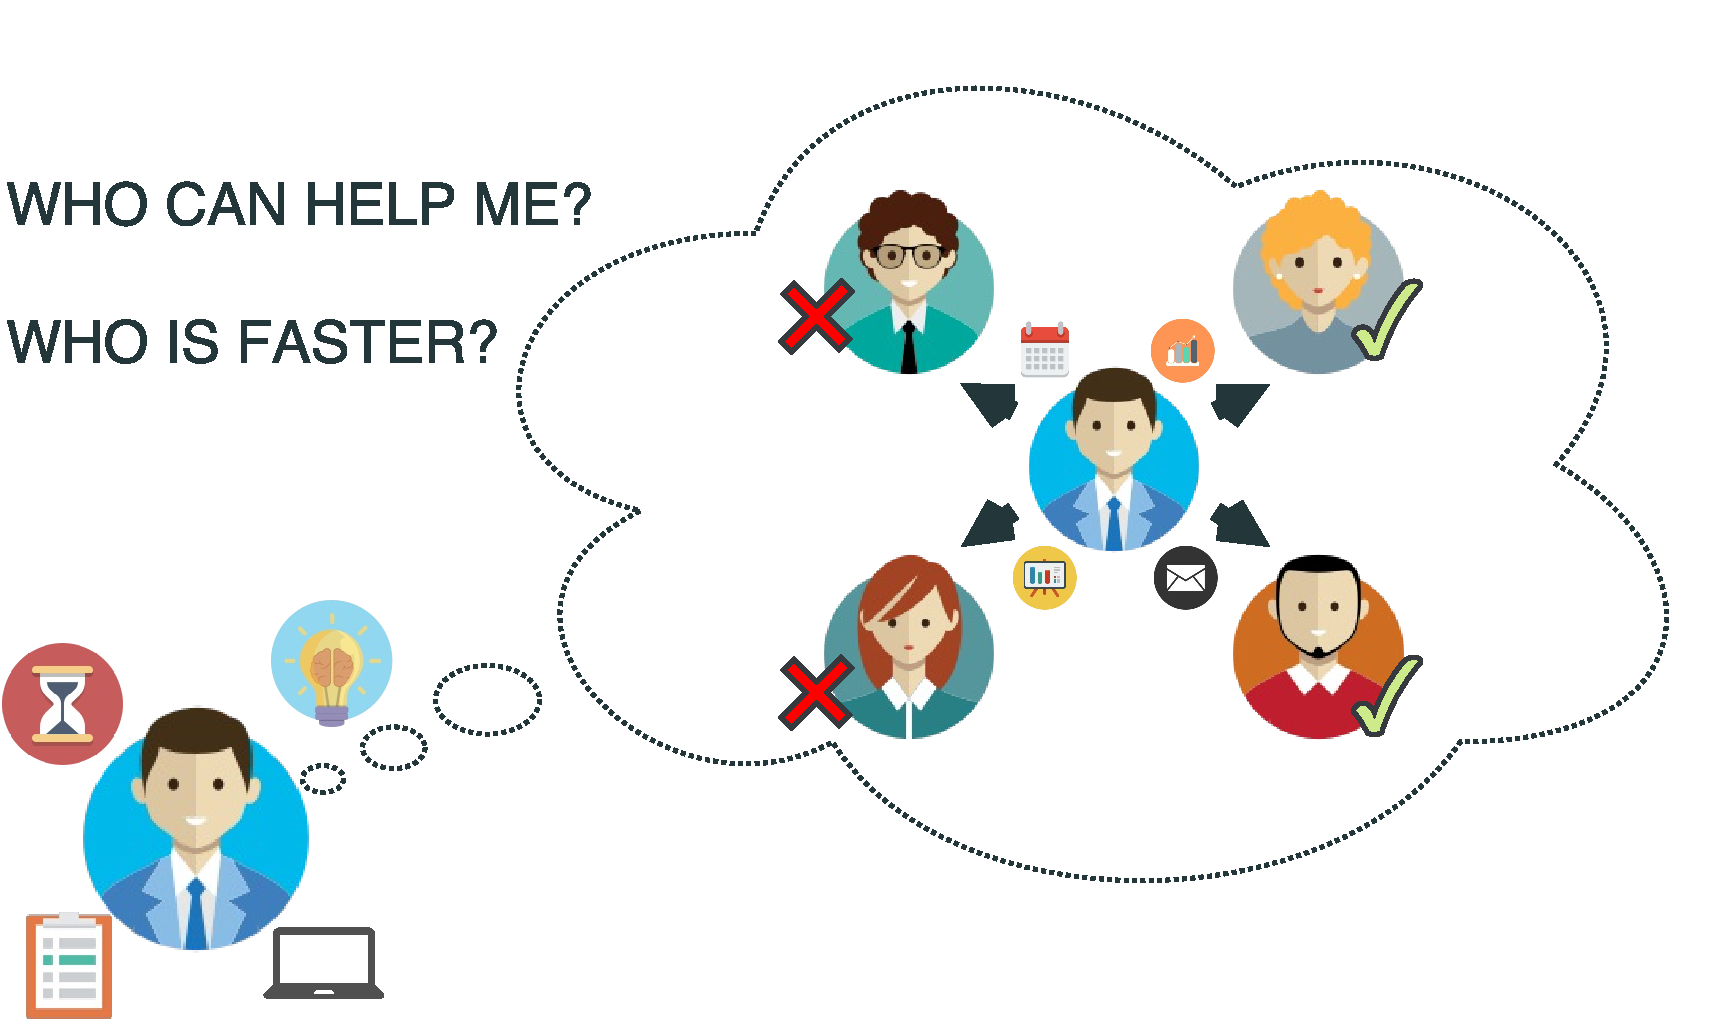
\includegraphics[width=\textwidth]{img/delegation.pdf}  
  \end{frame}
  \begin{frame}{How should tasks be offloaded?}
    \begin{itemize}
    	\item MEC offloading orchestration is a complex problem
    	\item There is not a unified abstraction about offloading mechanisms
    	\item Current strategies are performance unaware
    	\item SDN \& KDN could help
    \end{itemize}
    \footnotesize{\textit{\\~\\MEC = Mobile Edge Computing, SDN = Software Defined Networking,\\KDN = Knowledge Defined Networking}}
  \end{frame}
  \begin{frame}{Offloading architecture}
	\begin{itemize}
		\item Architecture abstraction definition to address the complexity problem
		\item Knowledge Plane to support network management
		\item Performance aware traffic steering
	\end{itemize}
  \end{frame}
  \begin{frame}{Talk overview}
	\tableofcontents[hideallsubsections]
  \end{frame}
\section{Offloading Architecture}
\subsection{Abstraction}
	\mytoc
	\begin{frame}{Offloading architecture}
		\centering
		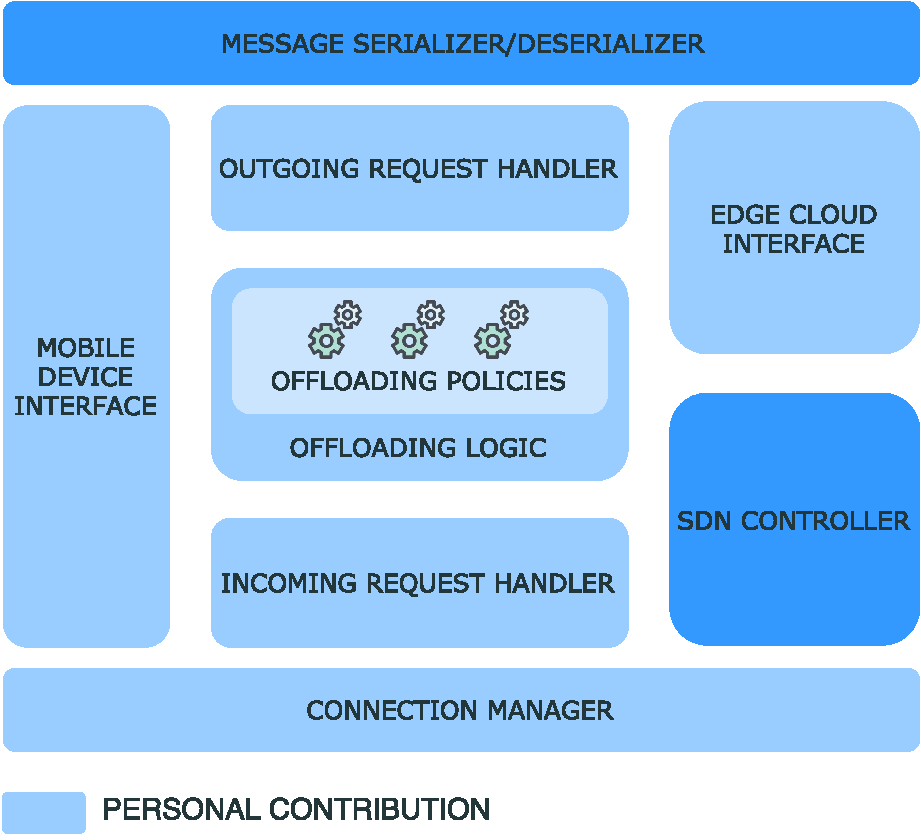
\includegraphics[scale=0.5]{img/off_sys_arch.pdf}
	\end{frame}
\subsection{Task Offloading Protocol}
	\mytoc
	\begin{frame}{Task offloading protocol}
		\centering
		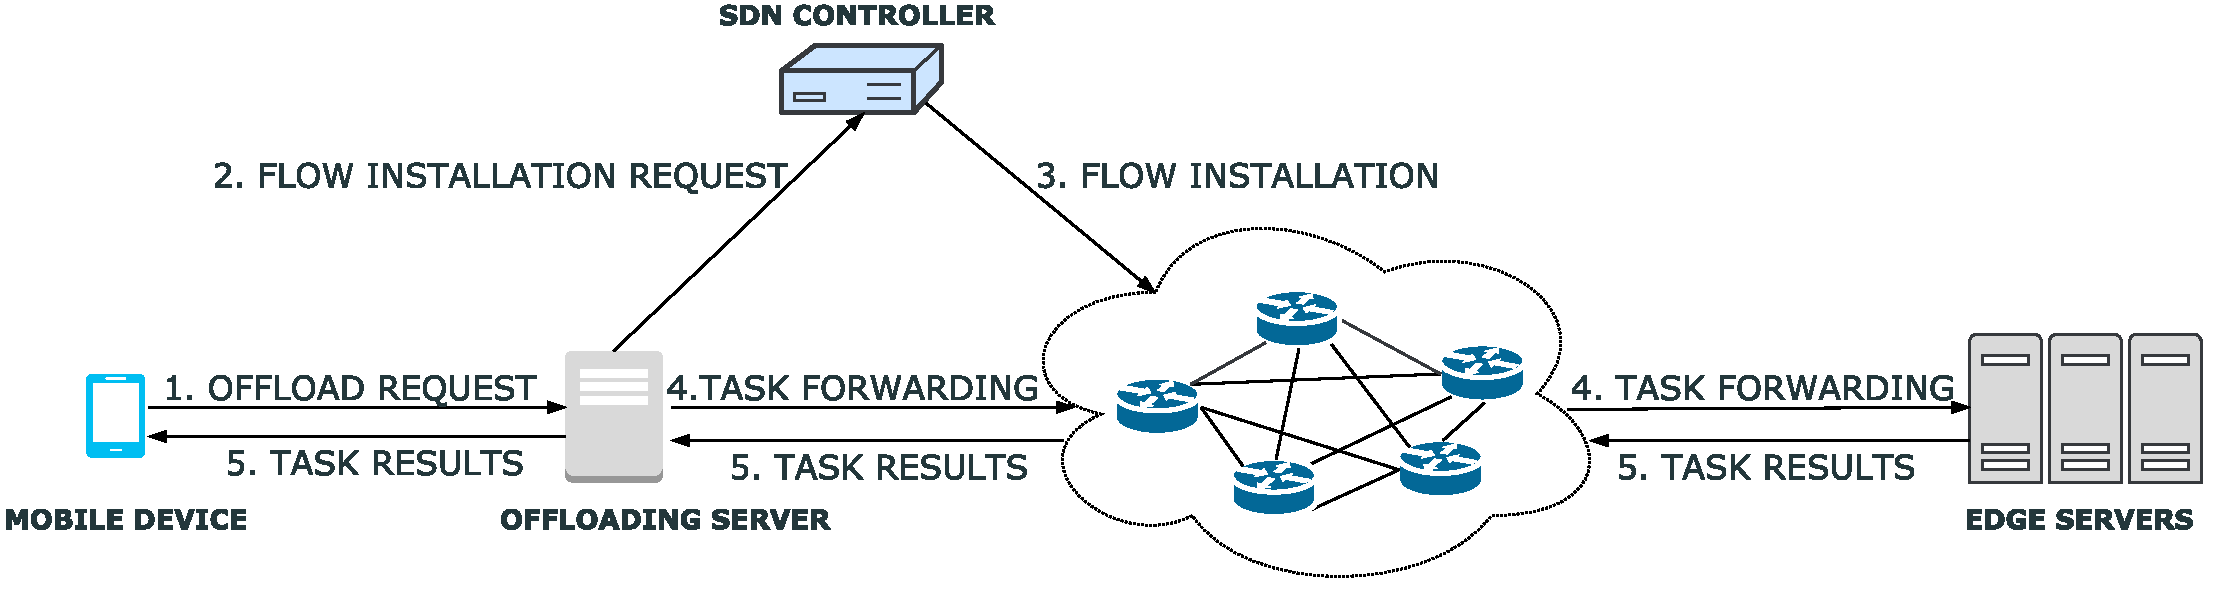
\includegraphics[scale=0.3]{img/protocol_sequence.pdf}
		\flushleft
		The protocol allows the client to specify:
		\begin{itemize}
		\item task requirements such as CPU, memory and latency
		\item offloading logic (e.g. LSTM path predictor, nearest server)
		\end{itemize}
	\end{frame}
\subsection{Path Prediction via LSTM}	
\subsubsection{Overview}
	\mytoc
	\begin{frame}{Path prediction via LSTM}
	Machine learning is a powerful tool for inference tasks
	\\~\\
	\centering	
	{\Huge$\Downarrow$}
	\flushleft
	\textbf{IDEA:} Routing problem as inference problem
	\end{frame}
	\frame{\frametitle{How to determine the best path?}Use traffic pattern as performance indicator.\\Perform path prediction with machine learning.\\~\\	
\centering
	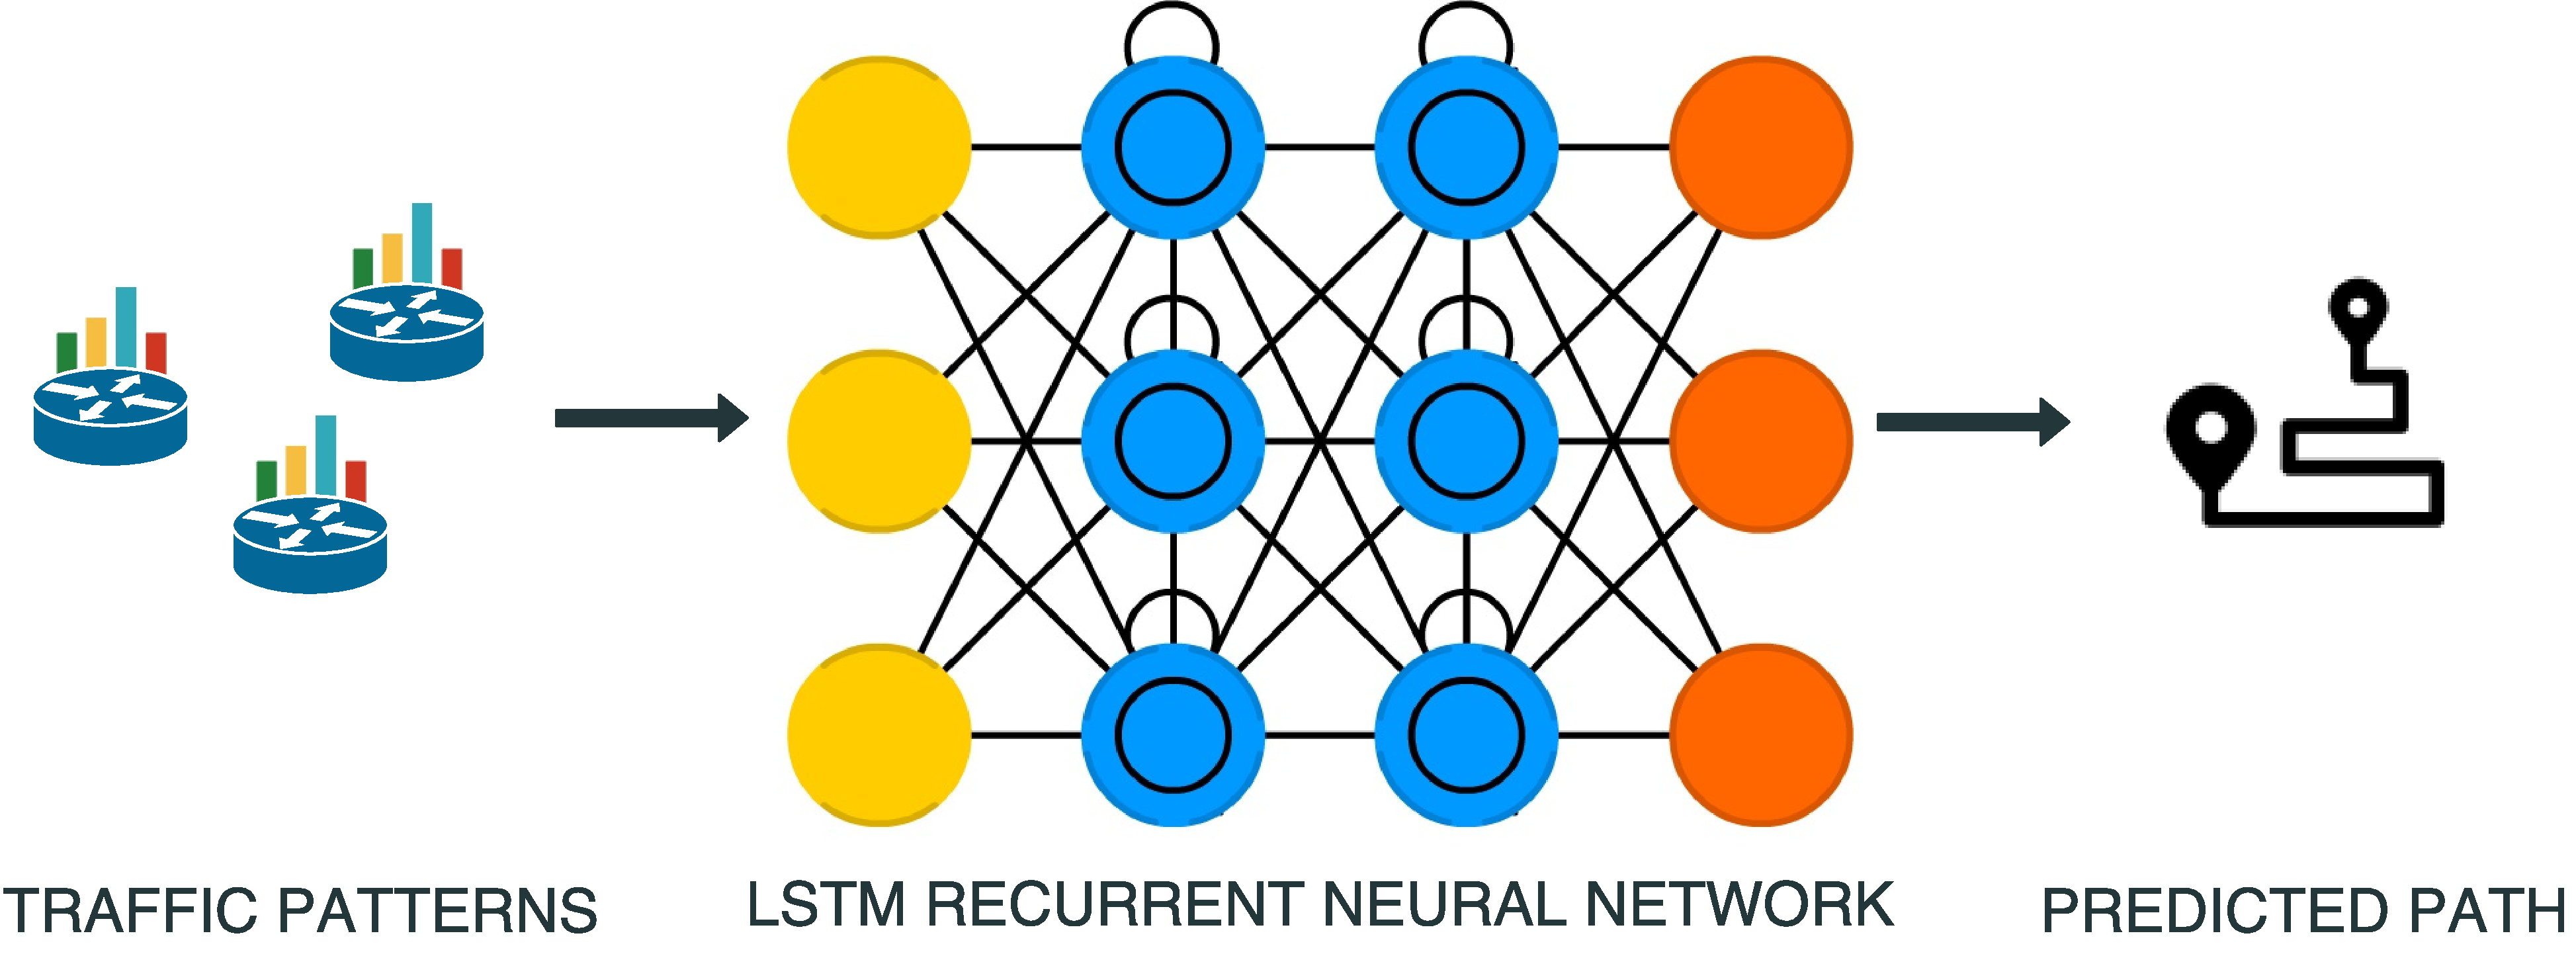
\includegraphics[width=\textwidth]{img/dnn.pdf}	
	}	
	\frame{\frametitle{Long Short-Term Memory (LSTM)}
	LSTM is an evolution of recurrent neural networks (RNNs) capable of memorizing data temporal patterns\\~\\
	\textbf{Objective:}\\Learn how traffic patterns evolve and route accordingly
	}
	\frame{\frametitle{Learning from who?}LSTM RNNs  are a supervised learning method, they require data to learn from.\\ 
	We use OSPF routing decisions as a ground truth.\\~\\
	\centering
	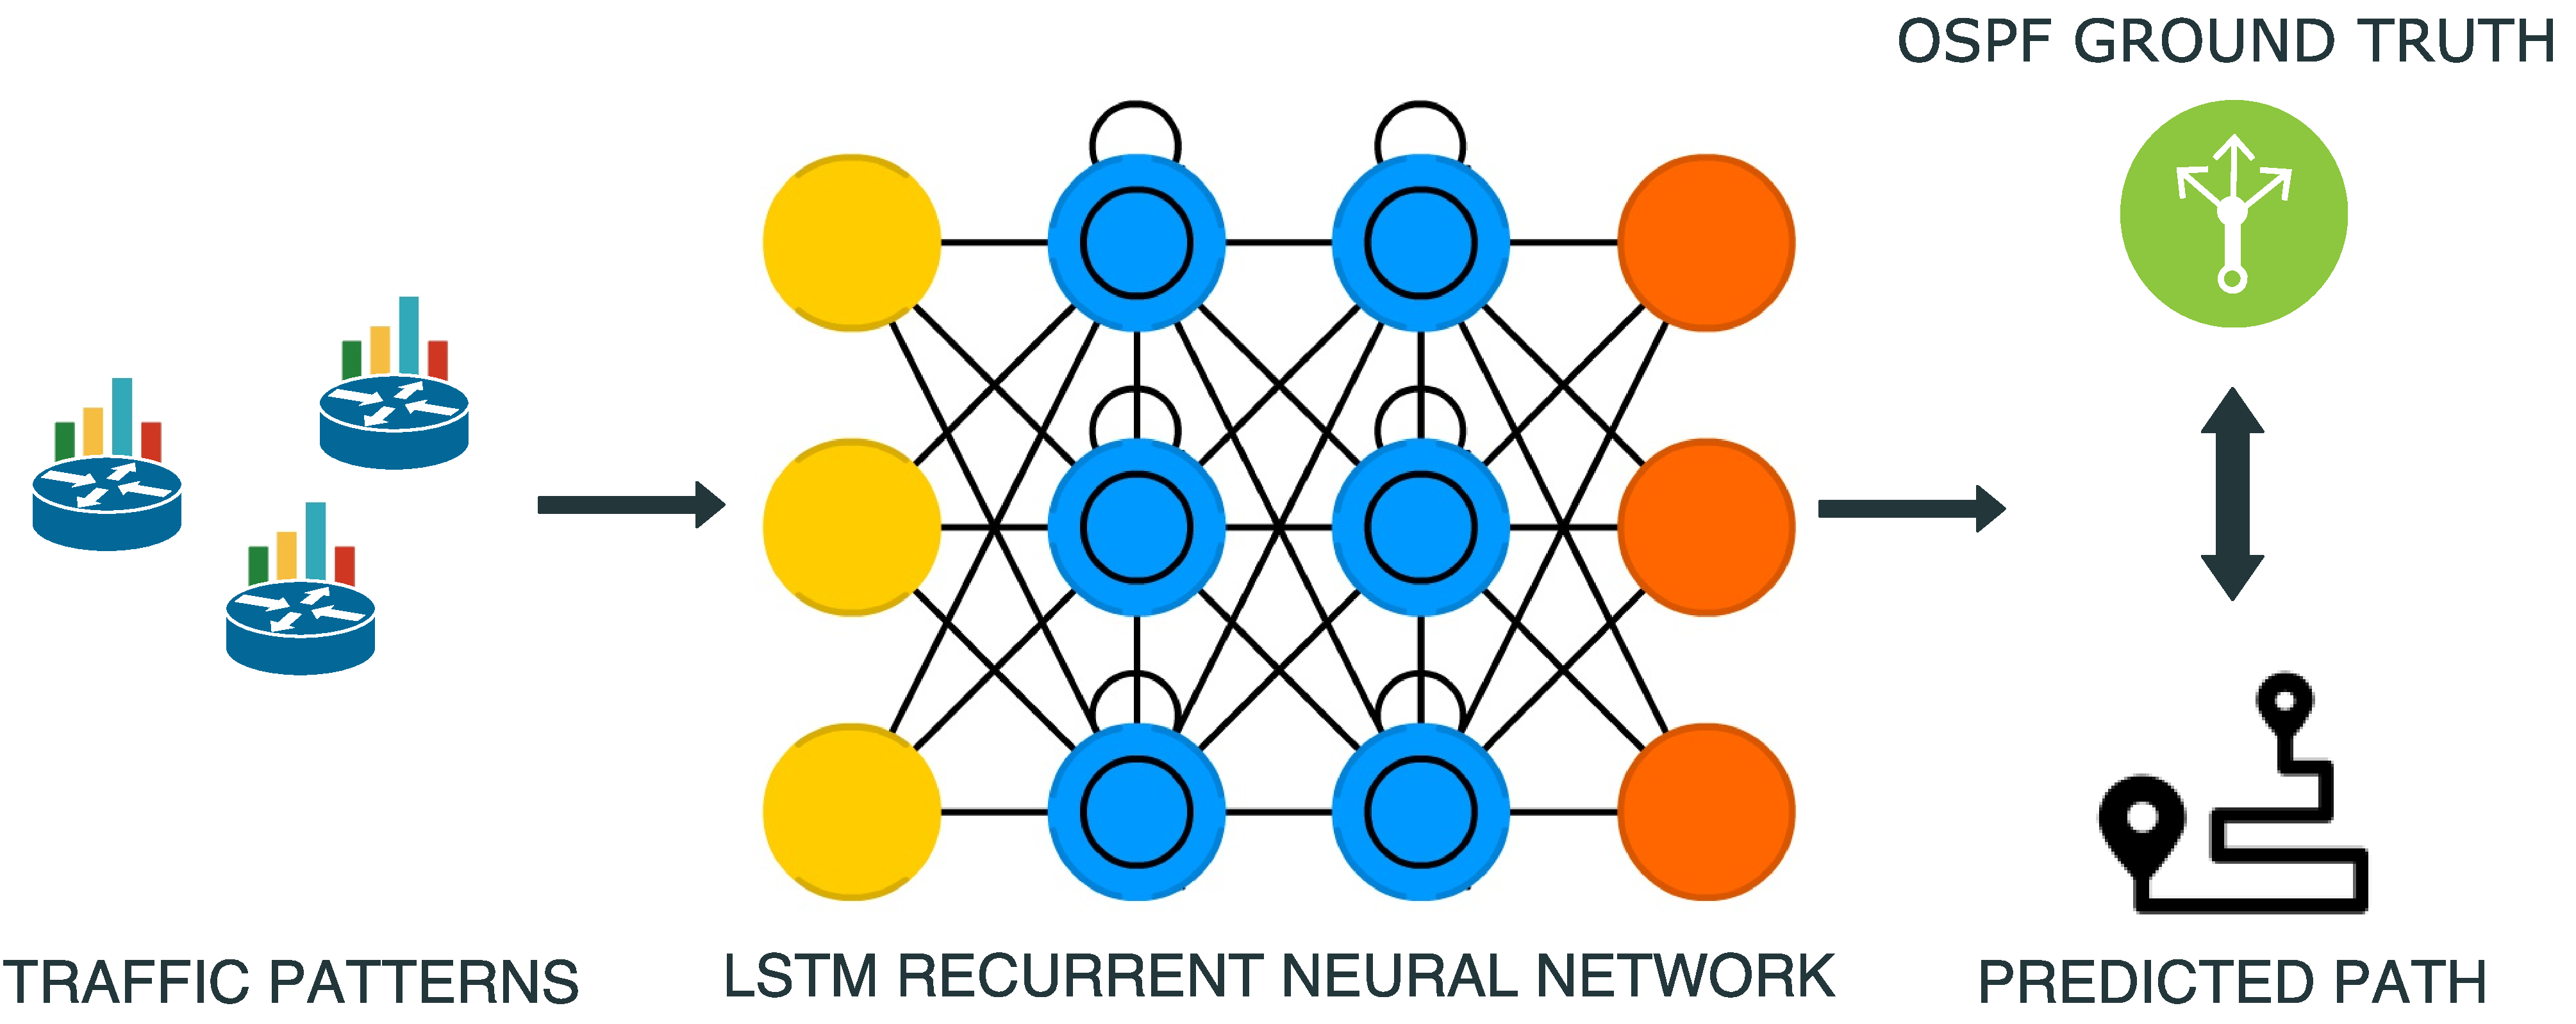
\includegraphics[width=\textwidth]{img/problem_model}
	}
	\frame{\frametitle{Problem formulation}	
	To use a LSTM we must define the model input and output.\\
	~\\
	\begin{columns}[totalwidth=\textwidth]
	\begin{column}{0.49\textwidth}
	\textbf{Input:}\\~\\
	Incoming packets count \\on each router\\~\\
	\end{column}
	\begin{column}{0.49\textwidth}  %%<--- here
	\textbf{Output:}\\~\\
	One-hot encoded vector \\with the next hop in the path\\~\\
\end{column}
\end{columns}
	\centering
	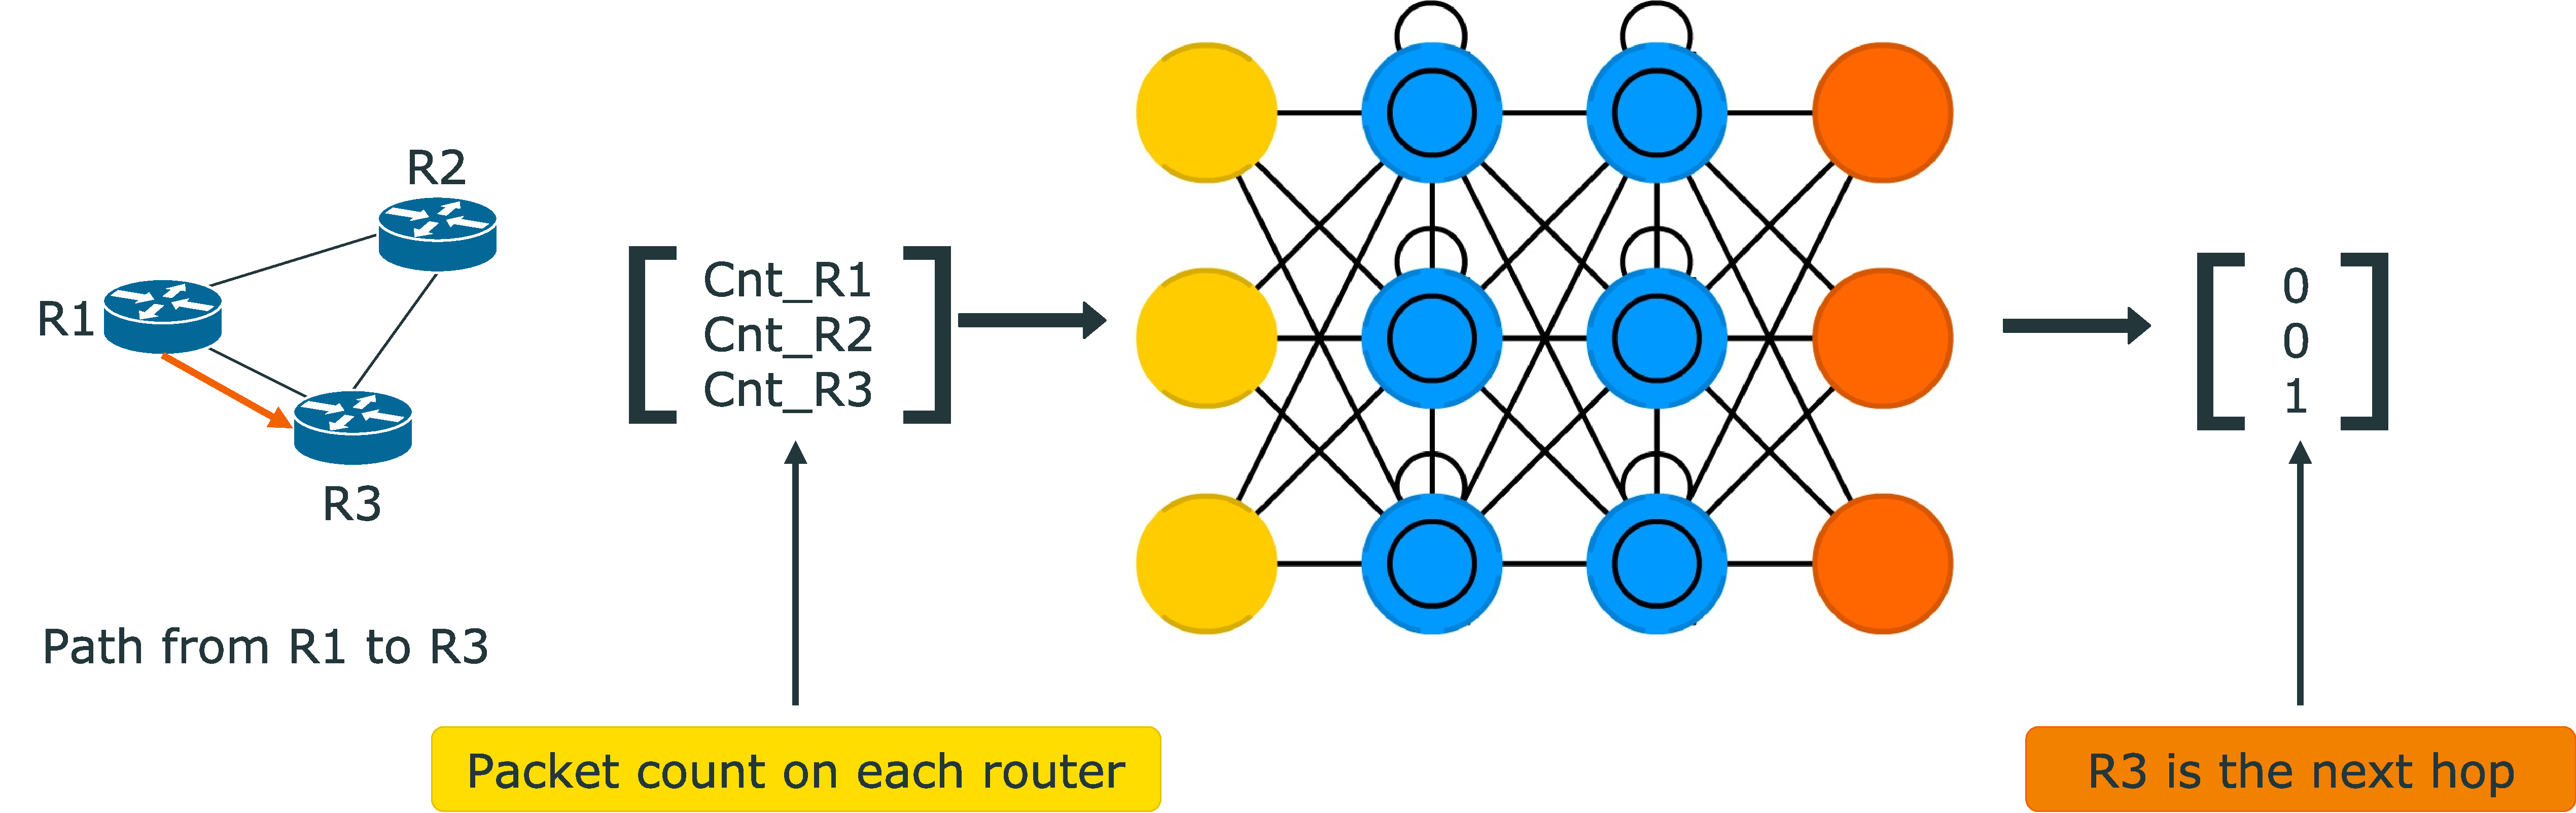
\includegraphics[width=\textwidth]{img/prediction_flow}
	}
	\frame{\frametitle{Path prediction process}Training a single model for all the targets in the topology is not feasible.\\~\\
	\textbf{SOLUTION}: train a model for all the source-destination pairs in the network.\\~\\
	To compute the whole path we iteratively use the model of the predicted next hop until the destination is reached.}
	\frame{\frametitle{Example: computing the path from R1 to R4 }	
	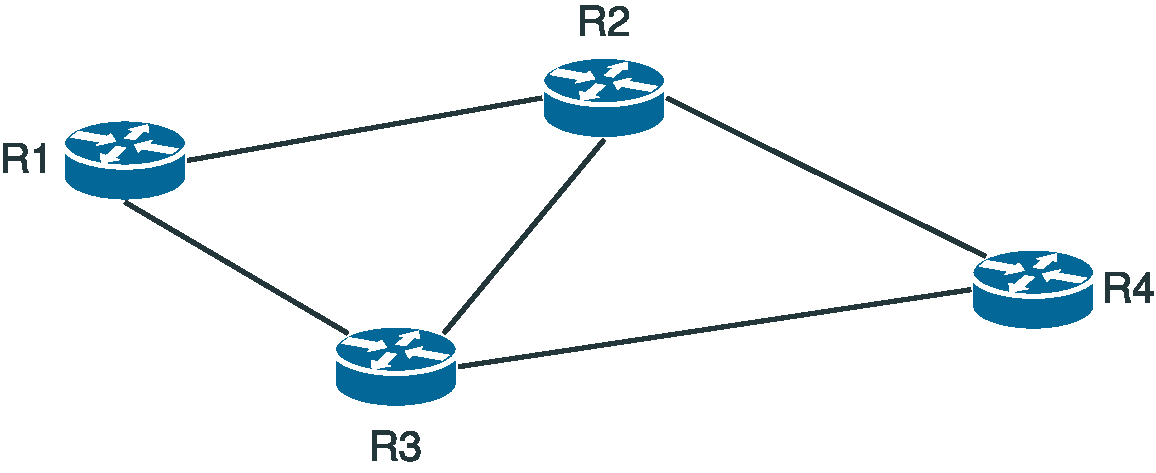
\includegraphics[width=\textwidth]{img/example.pdf}\\
	Step 1 - model = R1-R4 --> next hop = R2\\
	Step 2 - model = R2-R4 --> next hop = R3\\
	Step 3 - model = R3-R4 --> next hop = R4 \\~\\
	Computed path: R1 - R2 - R3 - R4\\}
	\subsubsection{Dataset}
	\mytoc
	\frame{\frametitle{Dataset generation}
	To train our model we need:
	\begin{itemize}
	\item network topology
	\item routing algorithm
	\item packet counter
\end{itemize}
	We could not find any public dataset suited to our needs so we create our own.
	}
	\frame{\frametitle{Network topology}
	We create this topology using MiniNeXt
	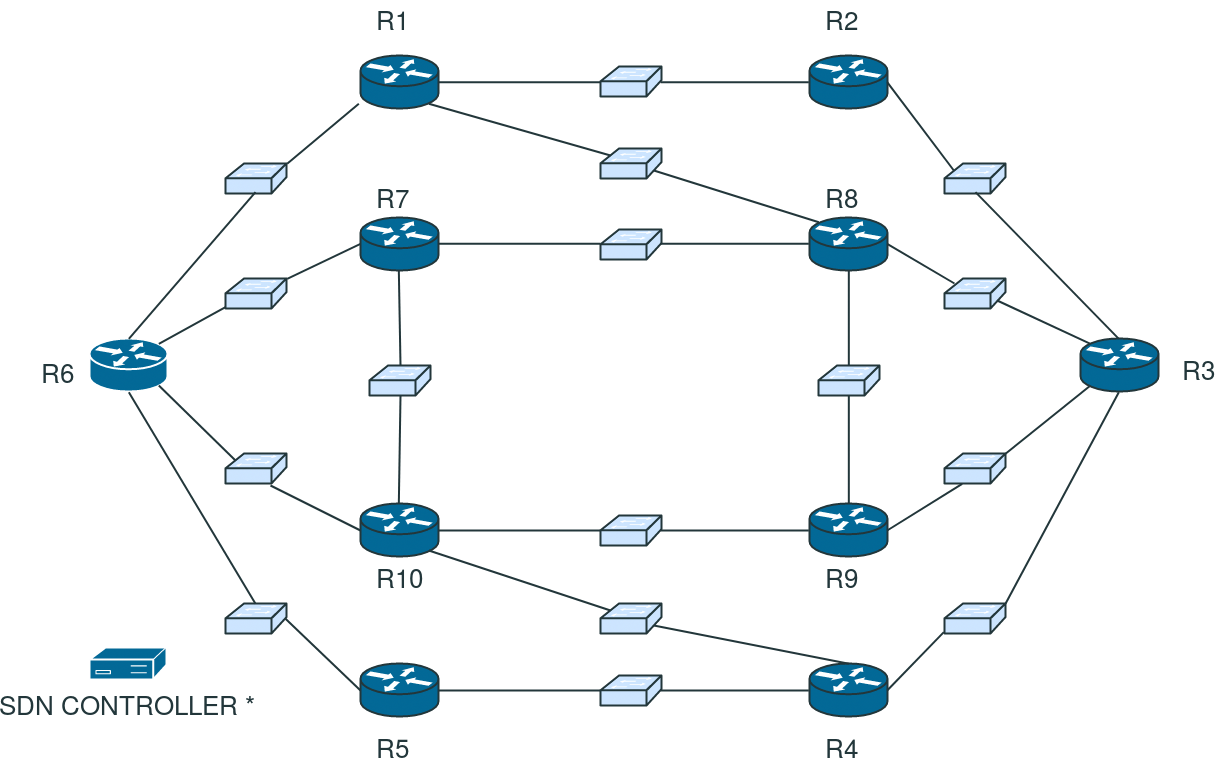
\includegraphics[width=\textwidth]{img/network_arch}\\ 
	\tiny{\textit{* All switches are connected to the SDN controller}}	
	}
	\frame{\frametitle{Routing algorithm}
	To run routing algorithms on MiniNeXt nodes we use Quagga.\\
	Quagga is a routing suite providing different routing algorithms (e.g OSPF, IS-IS, RIP).\\~\\
	We choose OSPF because of its wide adoption as iBGP.\\
	We also take in consideration Equal-Cost Multi Path (ECMP) to compare the performance.
	}
	\frame{\frametitle{Packet counter}
	The SDN controller --Ryu-- is responsible of retrieving the packet count.\\~\\
	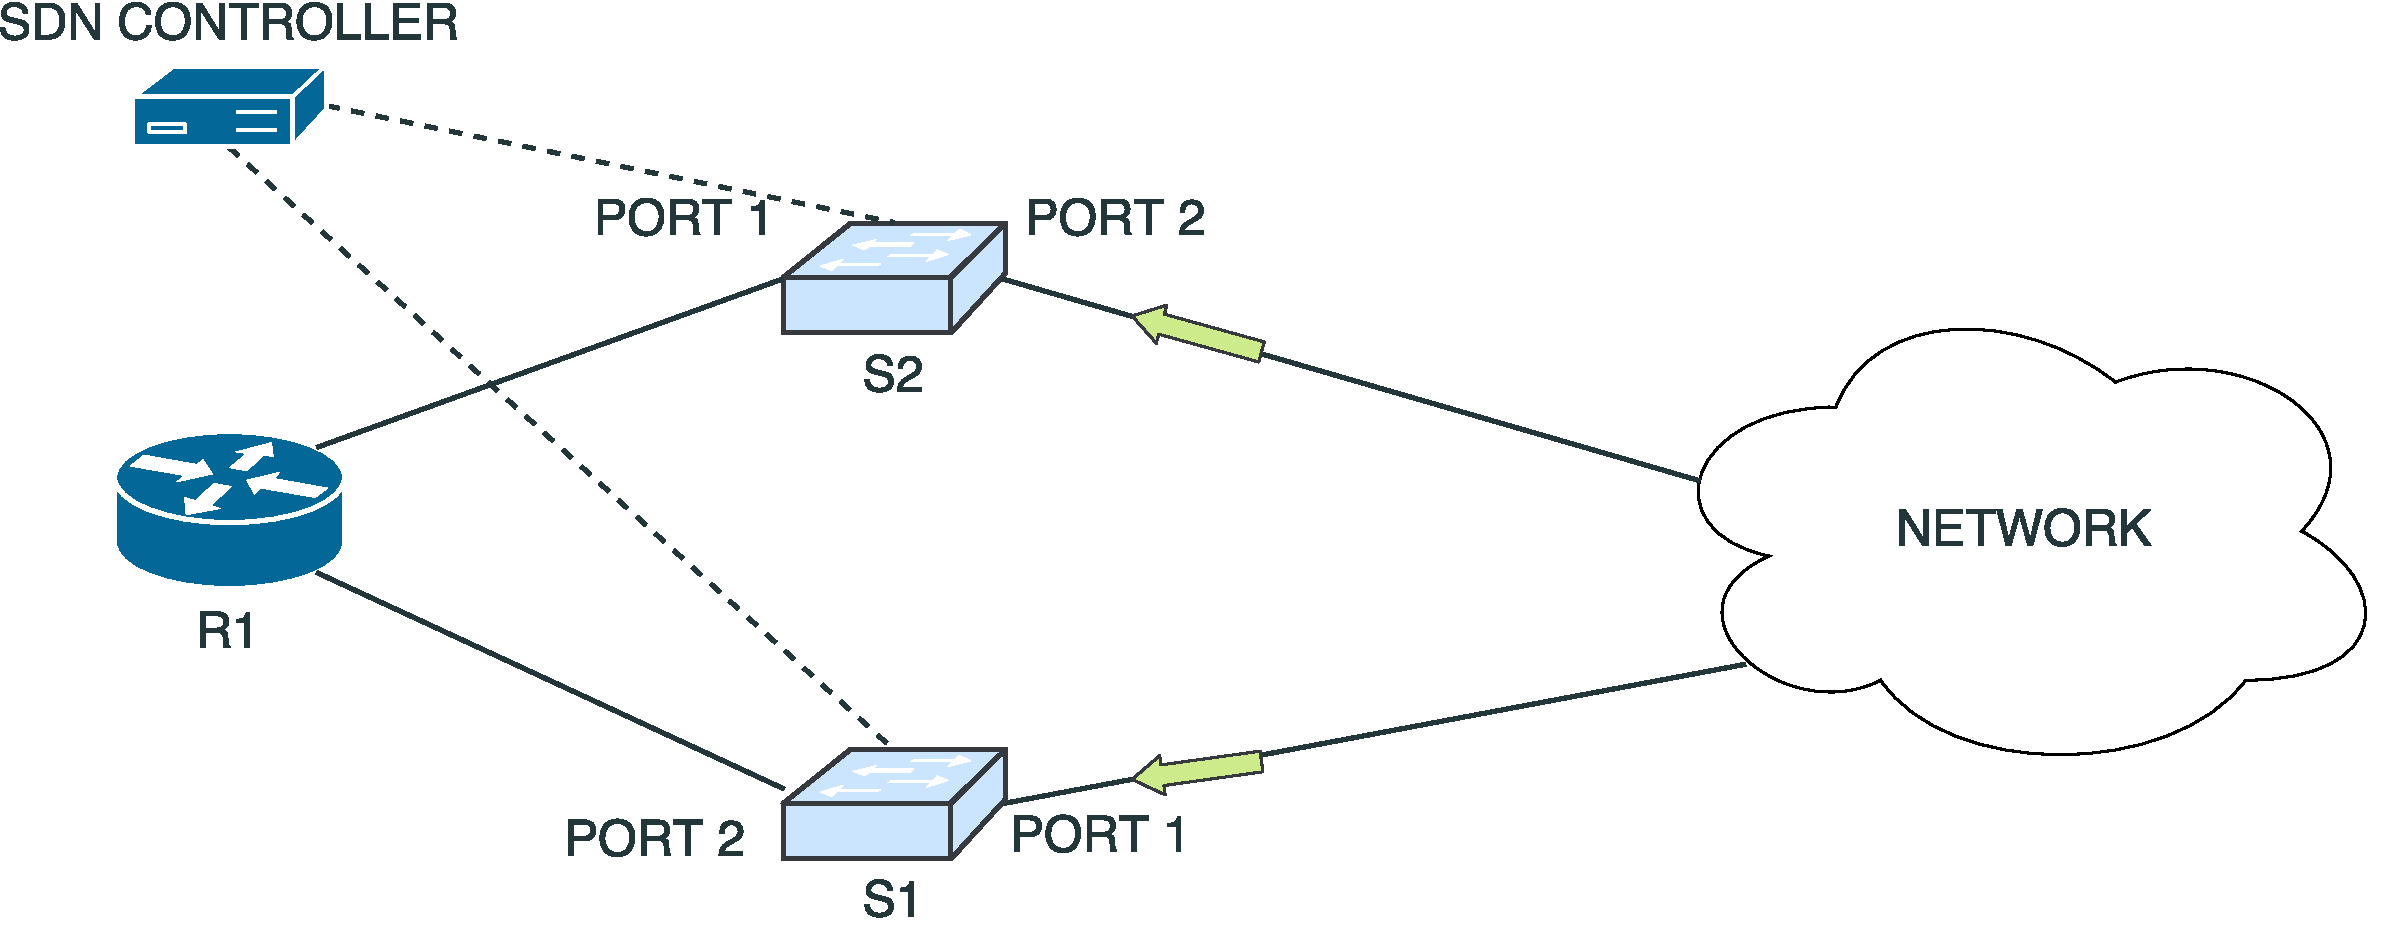
\includegraphics[width=\textwidth]{img/packet_counter.pdf}
	}
		
	\frame{\frametitle{Dataset generation steps}
		\MyArrow[1.3em]{start}{end}{line width=1pt}[out=150, in=210]	

	\begin{itemize}
	\item~\tikzmark{end}Initialize the topology with different link speed
	\item Simulate traffic for a certain duration
	\item Save packet count and routing tables
	\item~\tikzmark{start}Stop the traffic simulation and tear down the network
	% ADD ARROW FROM THE LAST TO THE FIRST BULLET
	\end{itemize}
	}
	
	\subsubsection{LSTM Architecture}
	\mytoc
	\frame{\frametitle{How to decide the LSTM structure?}
	The number of layers and neurons cannot be decided a priori.
	Cross validation is a powerful technique to determine the model parameters.\\~\\
	We test 24 configurations and average the results of 10 runs.\\~\\
	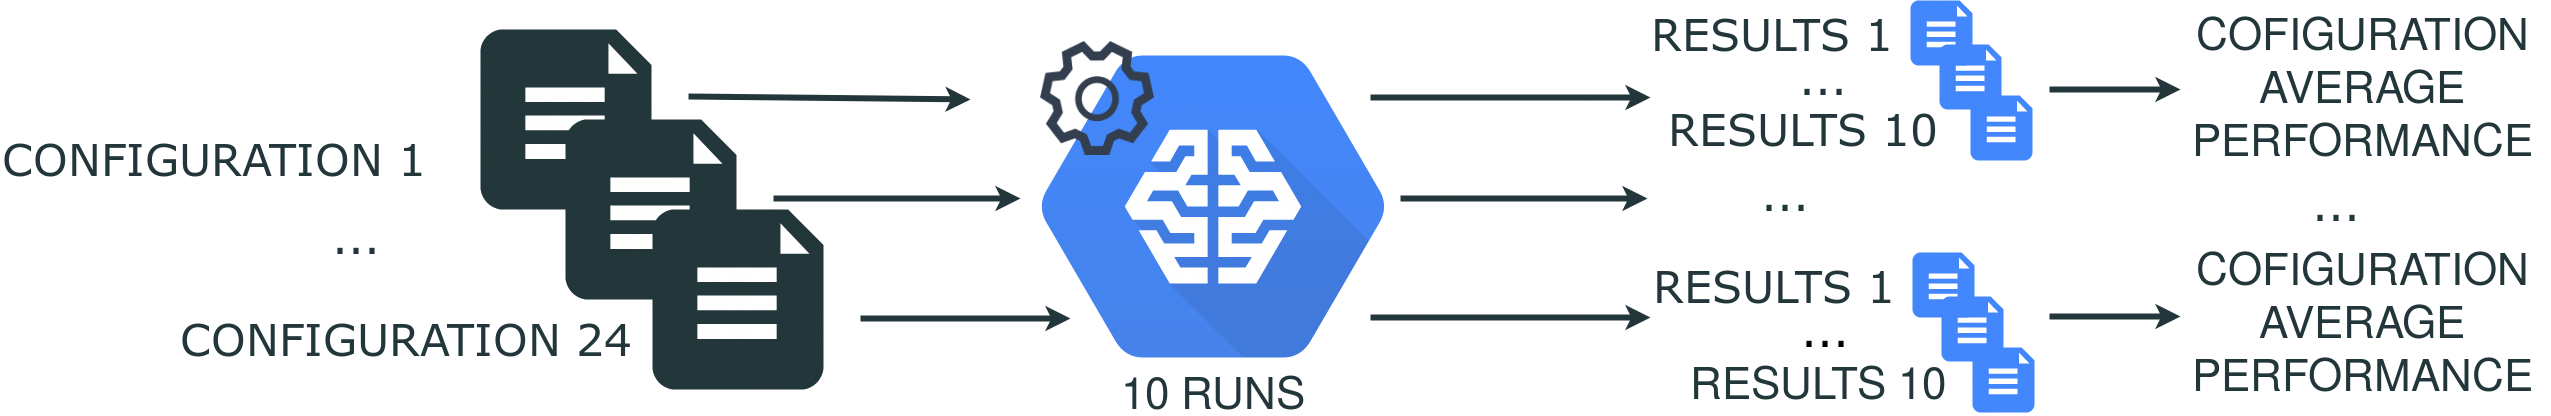
\includegraphics[width=\textwidth]{img/cross_validation}
	}
	\frame{\frametitle{Accuracy: more neurons or more layers?}
	Neurons affect performance more than hidden layers\\~\\	
	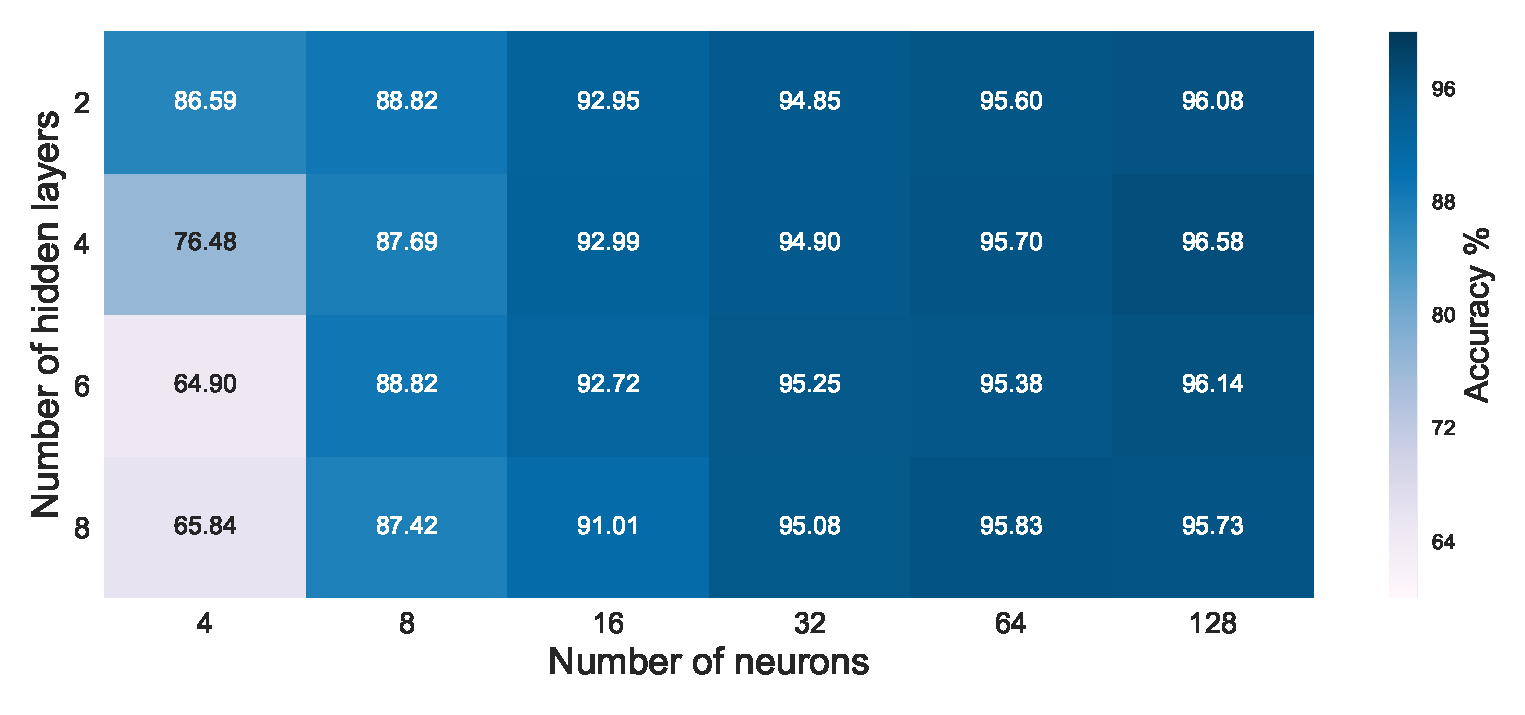
\includegraphics[width=\textwidth]{img/architecture_cmp}	
	}
	
	\frame{\frametitle{Finding the compromise: training time}
	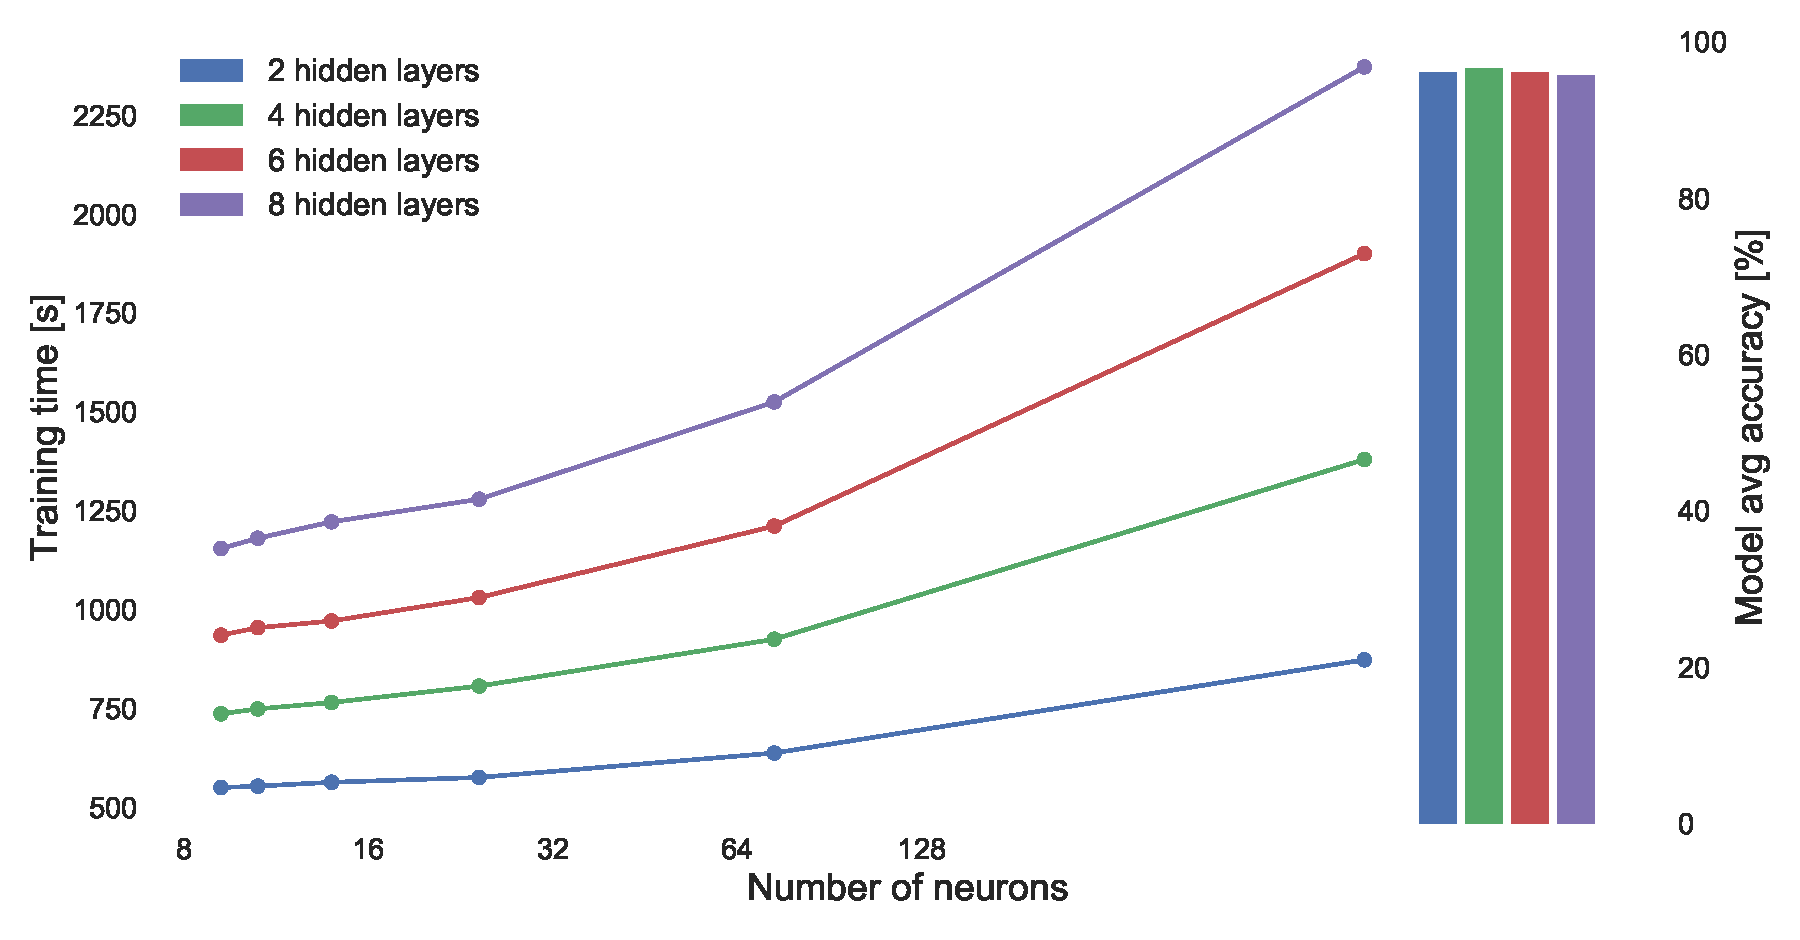
\includegraphics[width=\textwidth]{img/timing_cmp}	\\~\\
	\tiny{\textit{* Accuracy shown only for models with 128 neurons}}	
	}
	\frame{\frametitle{Tuning the network: input normalization}
	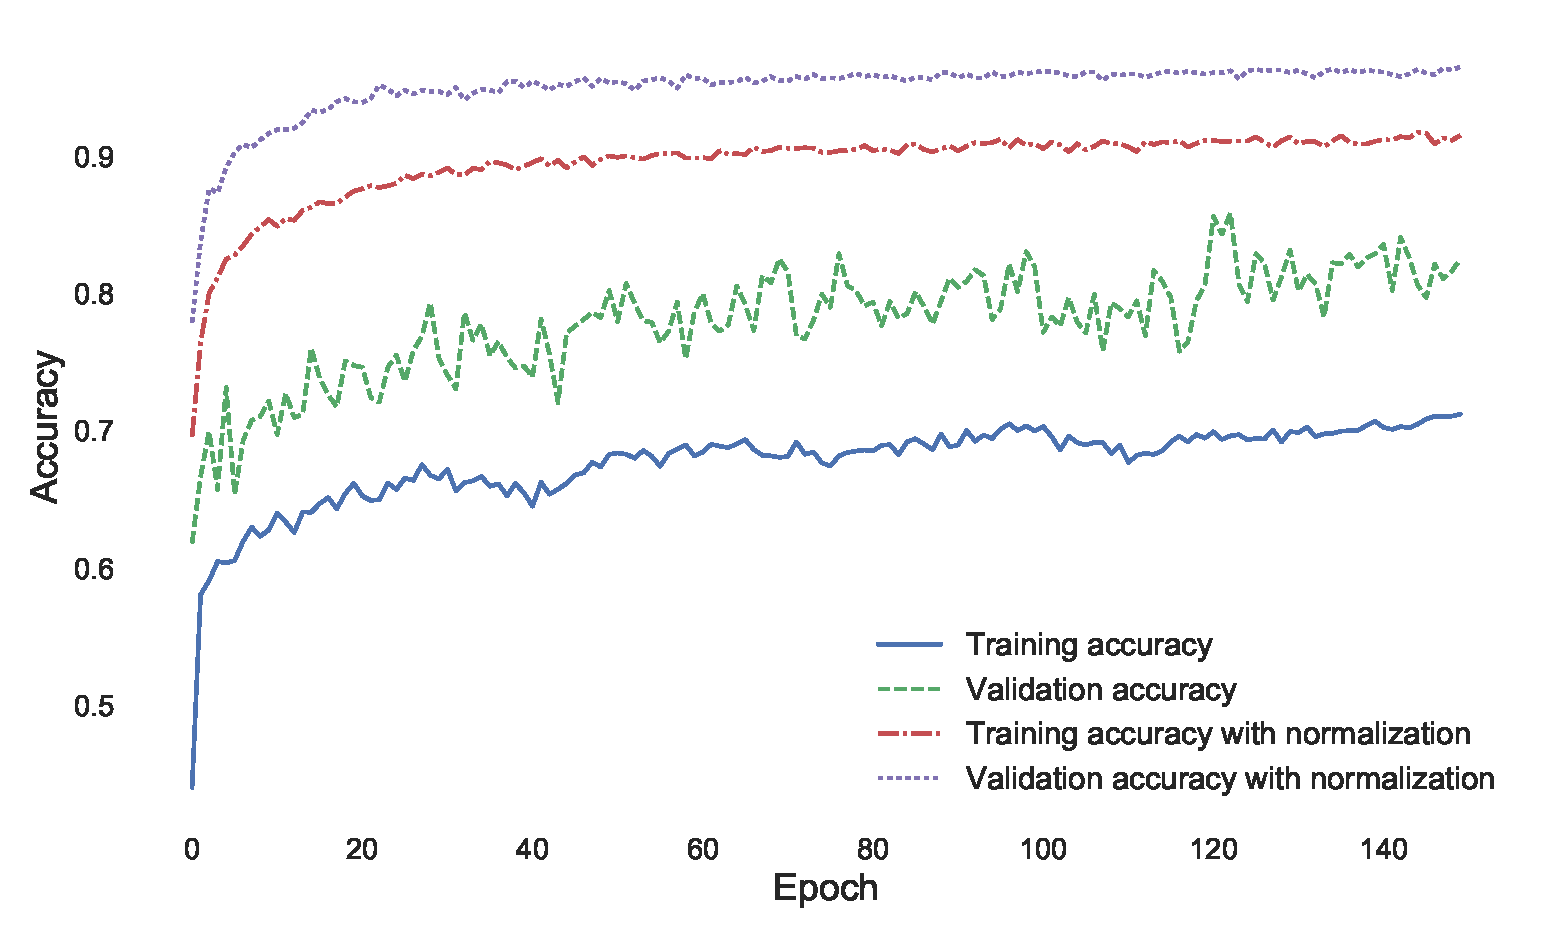
\includegraphics[width=\textwidth]{img/normalization_acc_cmp}	\\~\\
	\tiny{\textit{* Accuracy shown only for models with 128 neurons}}	
	}
	


\section{Results}
	\mytoc
	\frame{\frametitle{The system is able to emulate OSPF}
	We test the system's ability to behave like OSPF by averaging the performance of all the models on the test set.\\~\\The LSTM achieves an average accuracy of \textbf{98.71\%}.}% and a loss of only \textbf{0.0496}.}
	\frame{\frametitle{Is the system performance aware?}
	%We want to investigate the system ability to detect and adapt to network anomalies.\\
	We select a target and analyze, through an example, how our system behaves differently from OSPF in case of link loss.\\~\\
	\centering
	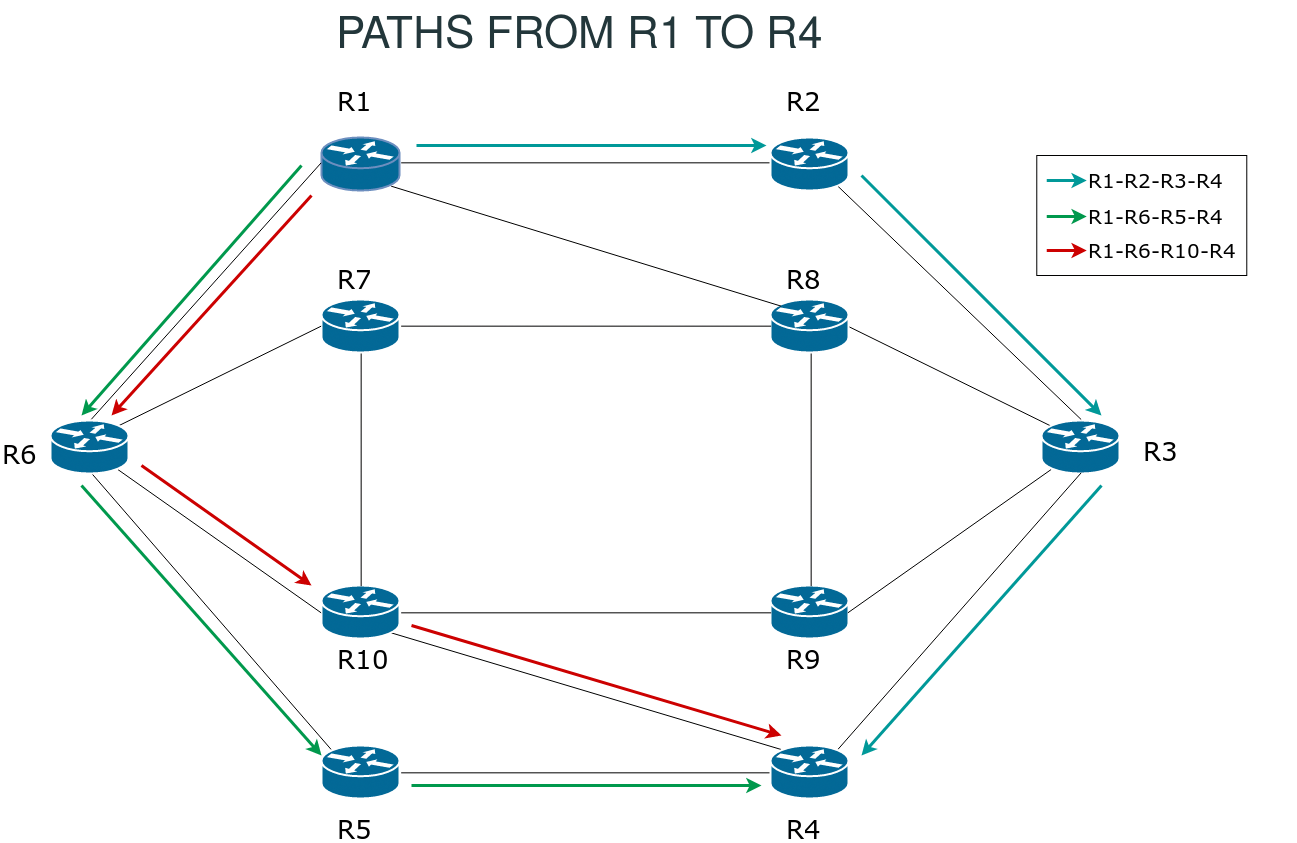
\includegraphics[scale=0.19]{img/validation_target}
	}
	\frame{\frametitle{The system exhibits a dynamic behavior}
	The LSTM path predictor is able to suggest multiple paths\\~\\
	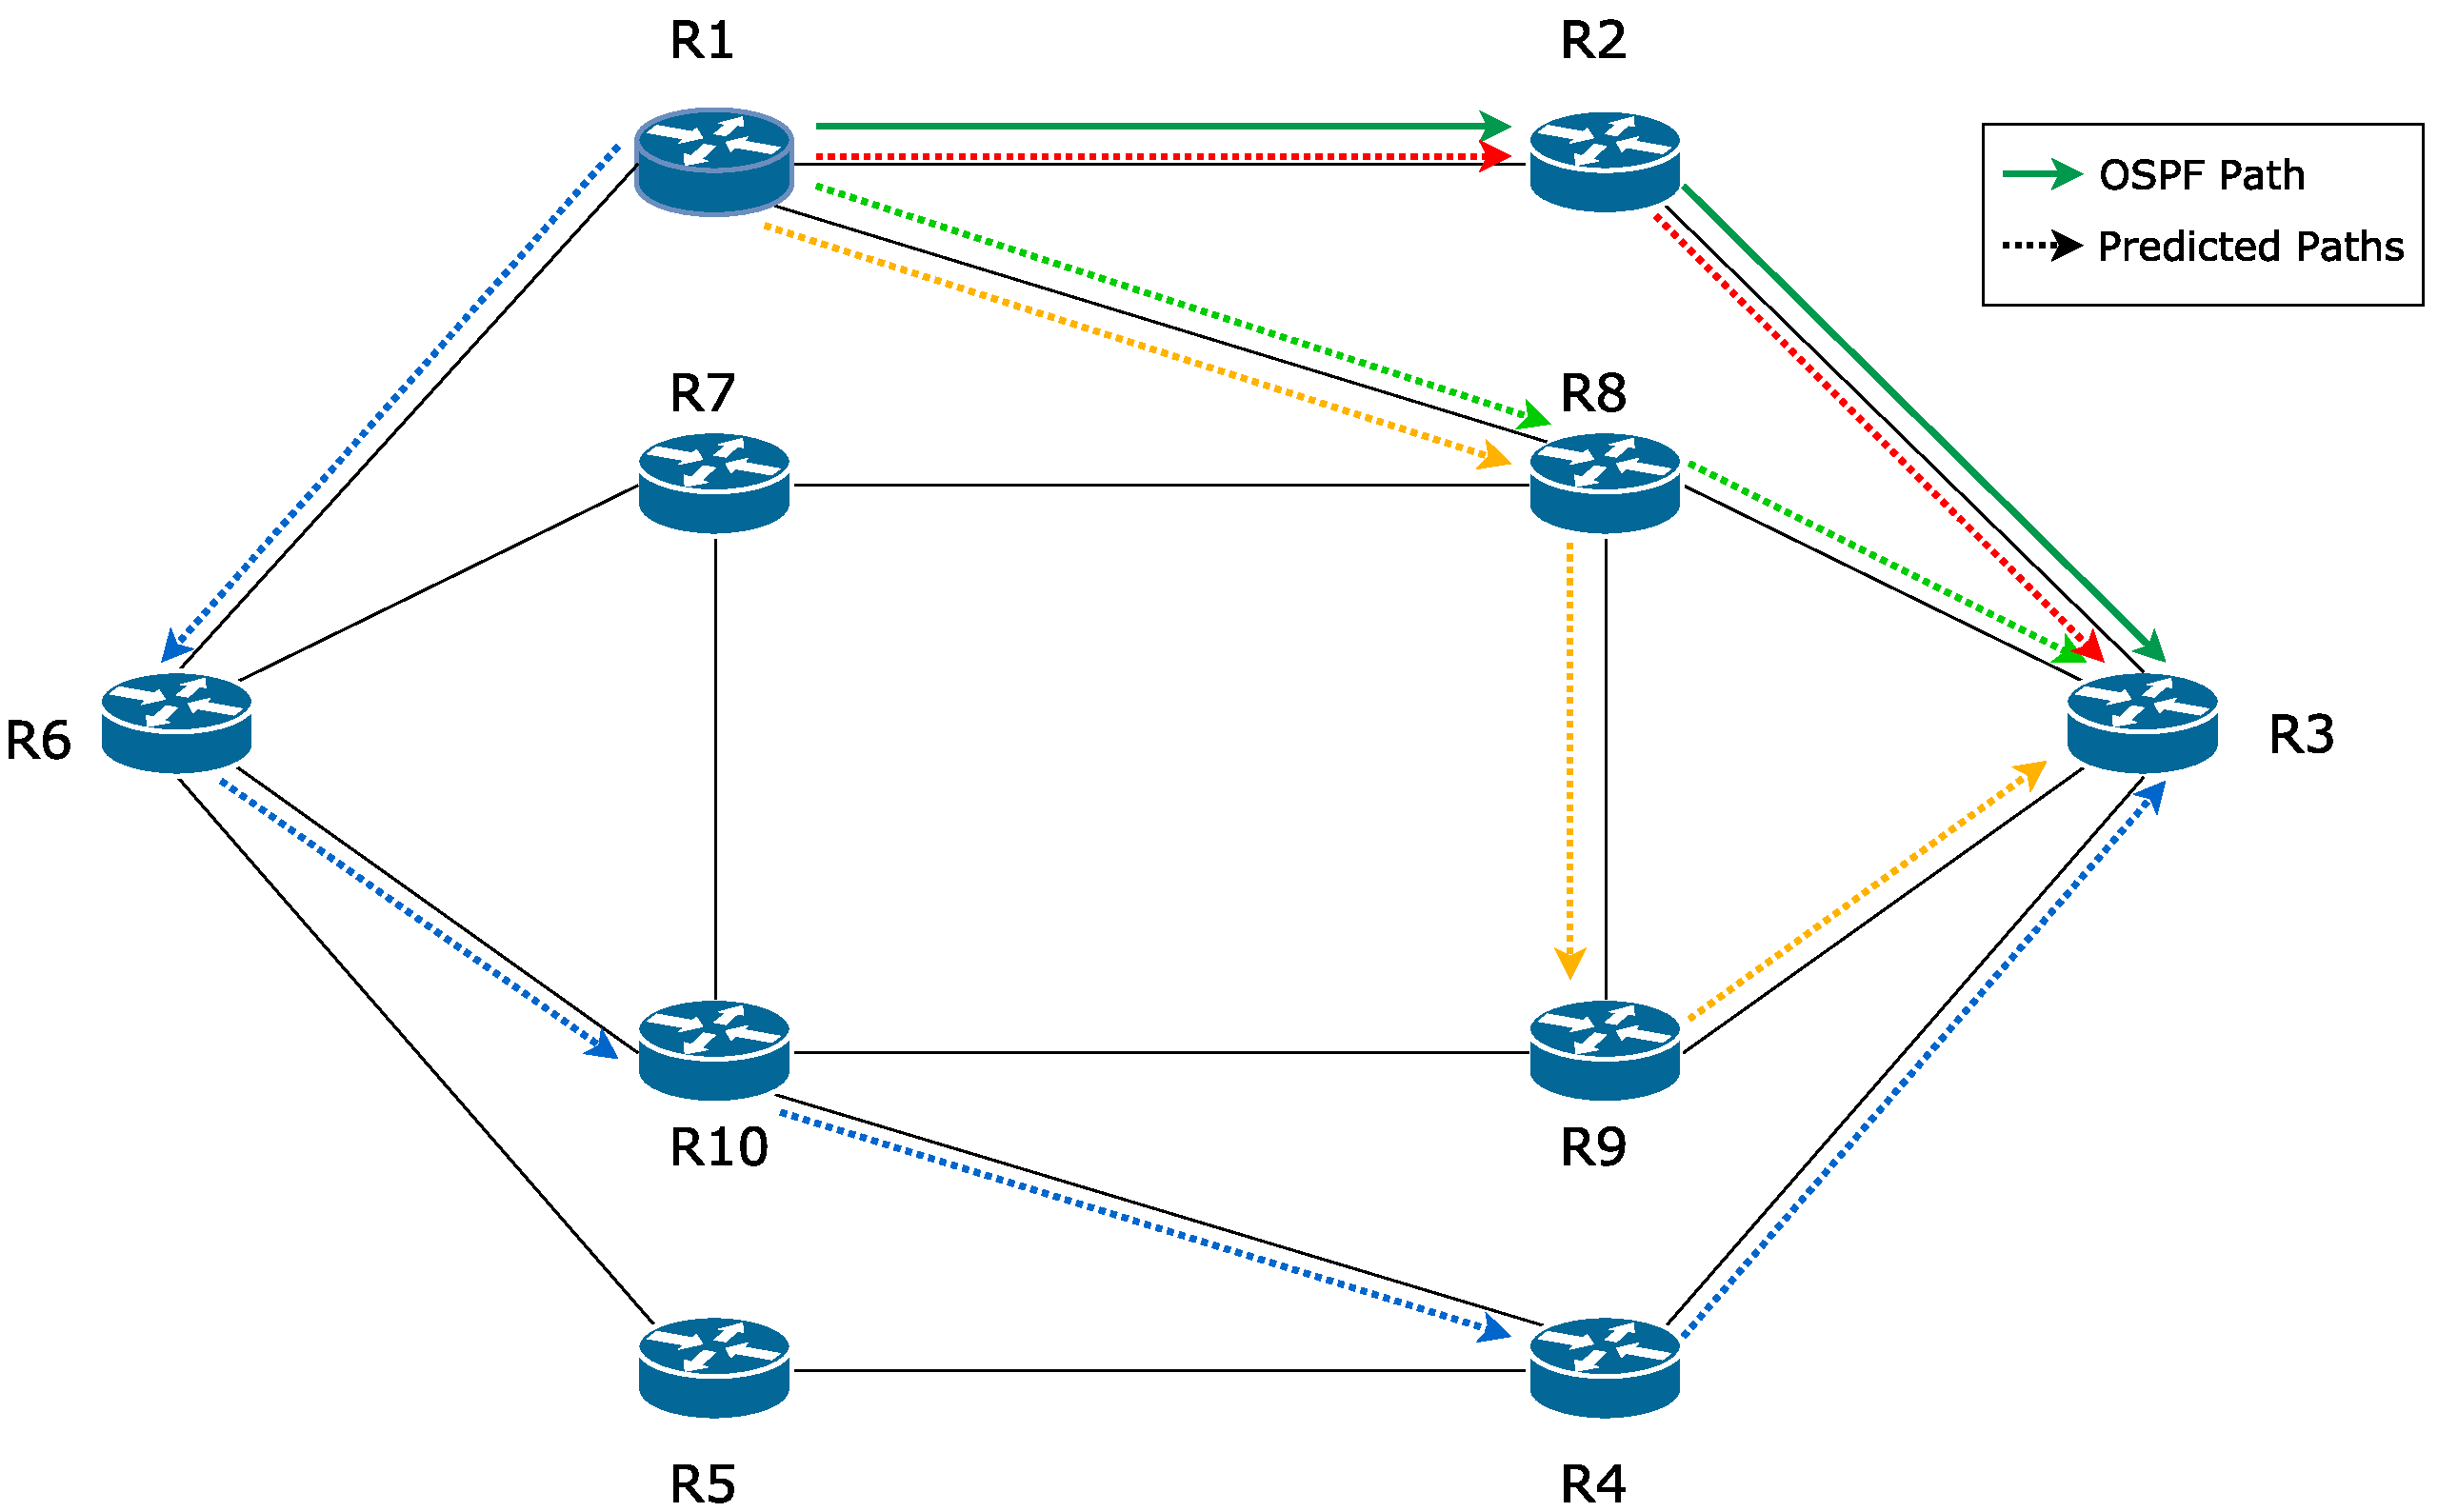
\includegraphics[width=\textwidth]{img/path_comparison}	
	}
	\frame{\frametitle{LSTMs outrun current approaches in terms of retransmission}
	In case of malfunctioning links, our system has a lower retransmission percentage then traditional routing\\~\\
	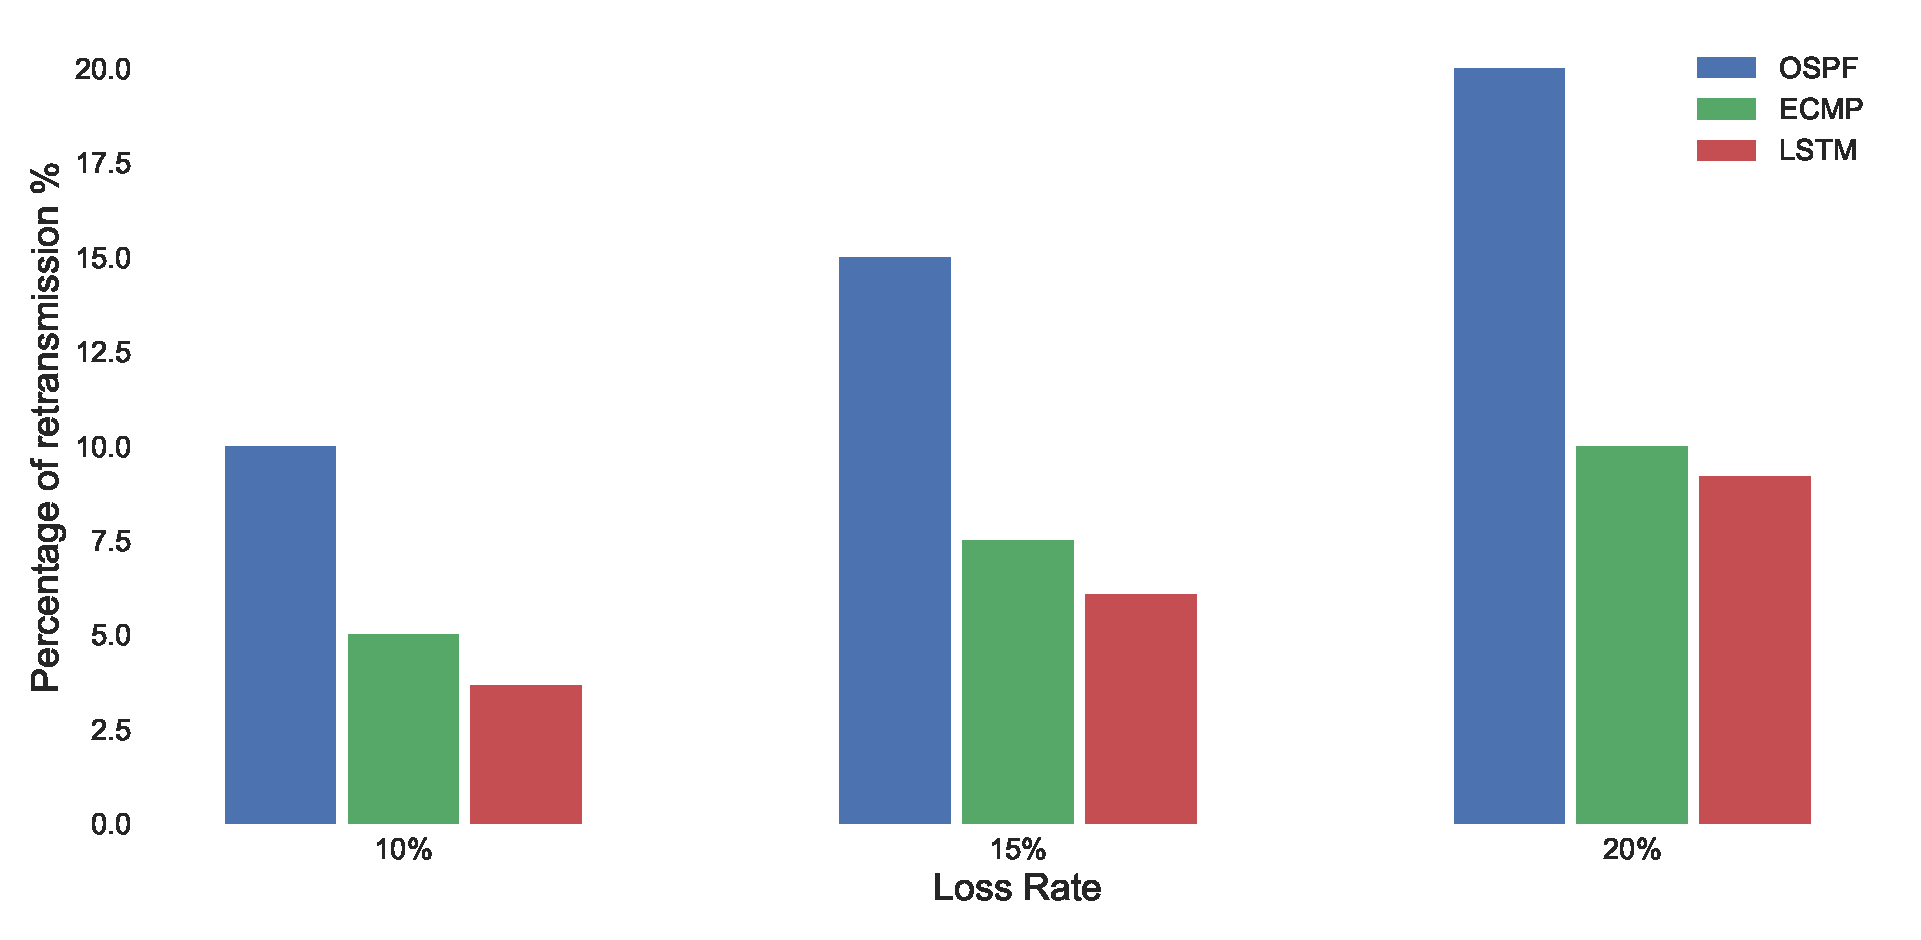
\includegraphics[width=\textwidth]{img/prediction_cmp_bar}\\
	\tiny{\textit{ECMP = Equal-Cost Multi Path, OSPF = Open Shortest-Path First, LSTM = Long Short-Term Memory
}	}}

\section{Limitations}
	\mytoc
	\begin{frame}{Limitations}
	Testbed:
	\begin{itemize}
	\item The functionalities of Mininet are limited
	\item The efficiency of the prediction system starts to decrease if the link loss is to high
	\end{itemize}
	Computation:	
	\begin{itemize}
	\item The training process is slow
	\item The number of models to train is big
	\item The controller needs GBs of memory to handle the trained models
	\end{itemize}
	\end{frame}
	\frame{\frametitle{Future work}
	The current results are encouraging, however, to further investigate the problem we aim to:
	\begin{itemize}
	\item get rid of Mininet emulation environment constraints  
	\item test the method on larger networks (e.g using GENI)
	\item run the testbed on a more scalable platform (e.g using GPU)
	\item explore more machine learning techniques \\(e.g reinforcement learning)
\end{itemize}		
	}
\section*{Take home messages}
\begin{frame}{Take home messages}
\begin{itemize}
\item	Mobile edge computing is a complex problem with no unified vision\\
\item	We prototyped an architecture for MEC offloading orchestration\\
\item	We developed a machine learning-based, performance aware routing strategy that improves on classic iBGP mechanisms
\end{itemize}	
	\end{frame}  
\frame{\titlepage}
\end{document}
